\chapter{Software Design}

\section{Architecture}
Monkey office is a web application deployed on a web server.
The application has two realms, front-end and back-end.
The front-end interacts with users directly though provided interfaces.
The system serves \gls{html} web pages to a client.
The client who access the system by a \gls{http} request with their web browser will receive a web page as a response.
The back-end is where the core of the system resides.
Because the system needs permanent storage to store data on request.
It needs to communicate with the database to store and retrieve data.
Figure \ref{fig:architecutre} shows overall subsystems and modules of the application.

\begin{landscape}
	\begin{figure}
		\centering
		\caption{Architecture of this system}
		\label{fig:architecutre}
		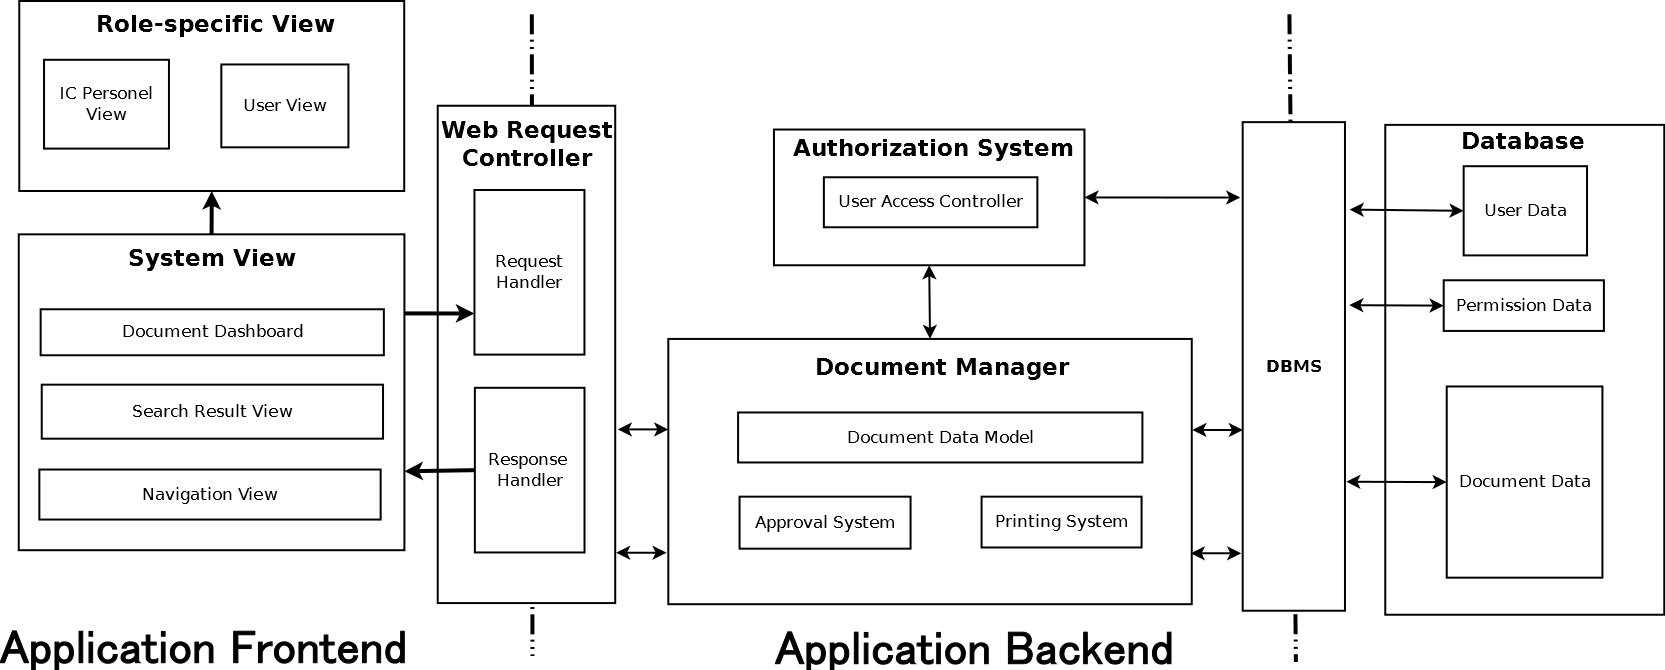
\includegraphics[scale=0.37]{res/software-design/monkeyOffice_architecture}
	\end{figure}
\end{landscape}

\subsection{Frontend}
Frontend consists of user interfaces called view.
It renders data received from application backend to users.
User can only interacts with the system through views only.
There are two types of view, system view and role-specific view.
System view is a base view available for all type of users.
It provides basic interaction functionality to the system such as search for documents, view documents, and navigating around the site.
Role-specific view extends the system view with some extra functionalities available only to specific type of users.
Those functionalities has already mentioned in section \ref{section:usecase}.
\gls{ic} personnel view available to staff, assistant of deputy dean, deputy dean, and dean only.
User view available to user only.
Table \ref{tbl:page-availability} shows all views in the system and their availability.

\begin{table}[h]
\centering
\caption{System views and their availability}
\label{tbl:page-availability}
\begin{tabular}{@{}lccC{2cm}ccL{3cm}@{}}
\toprule
\multirow{2}{*}{View} & \multicolumn{5}{c}{Availability}                                               & \multicolumn{1}{c}{\multirow{2}{*}{Description}} \\ \cmidrule(lr){2-6}
                      & User       & Staff      & Assistant of deputy dean & Deaputy dean & Dean       & \multicolumn{1}{c}{}                             \\ \midrule
Document Dashboard    & \checkmark & \checkmark & \checkmark               & \checkmark   & \checkmark & View lists of documents                          \\
Search Result         & \checkmark & \checkmark & \checkmark               & \checkmark   & \checkmark & View search result                               \\
Navigation            & \checkmark & \checkmark & \checkmark               & \checkmark   & \checkmark & Menu on the top to navigate around the site      \\
Document Approval     &            & \checkmark & \checkmark               & \checkmark   & \checkmark & Approve or reject documents                      \\
Document Printing     &            & \checkmark &                          &              &            & Print out documents                              \\ \bottomrule
\end{tabular}
\end{table}

\subsection{Backend}

\section{Storing Digital Documents}
Storing documents mean saving documents uploaded by users and create a metadata so that the system can access them.
The purpose of storing metadata is to create an abstract concept of the document.
According to requirements and use cases, the document should contain attachments and other related documents.
The document can be official or unofficial documents.
Both official and unofficial documents are the same except for one characteristic.
Official documents has a customized identification code as mentioned in table \ref{tbl-doc-subtype}.
Unofficial documents has only regular identification number starting at one and increment by one for each document.
Therefore, the parent document have to store a list of attachments.
That is a list referring to itself.
A class diagram in figure \ref{fig:doc-template} shows relationships between each unit.

\begin{figure}
	\caption{Document template creation class diagram}
	\label{fig:doc-template}
	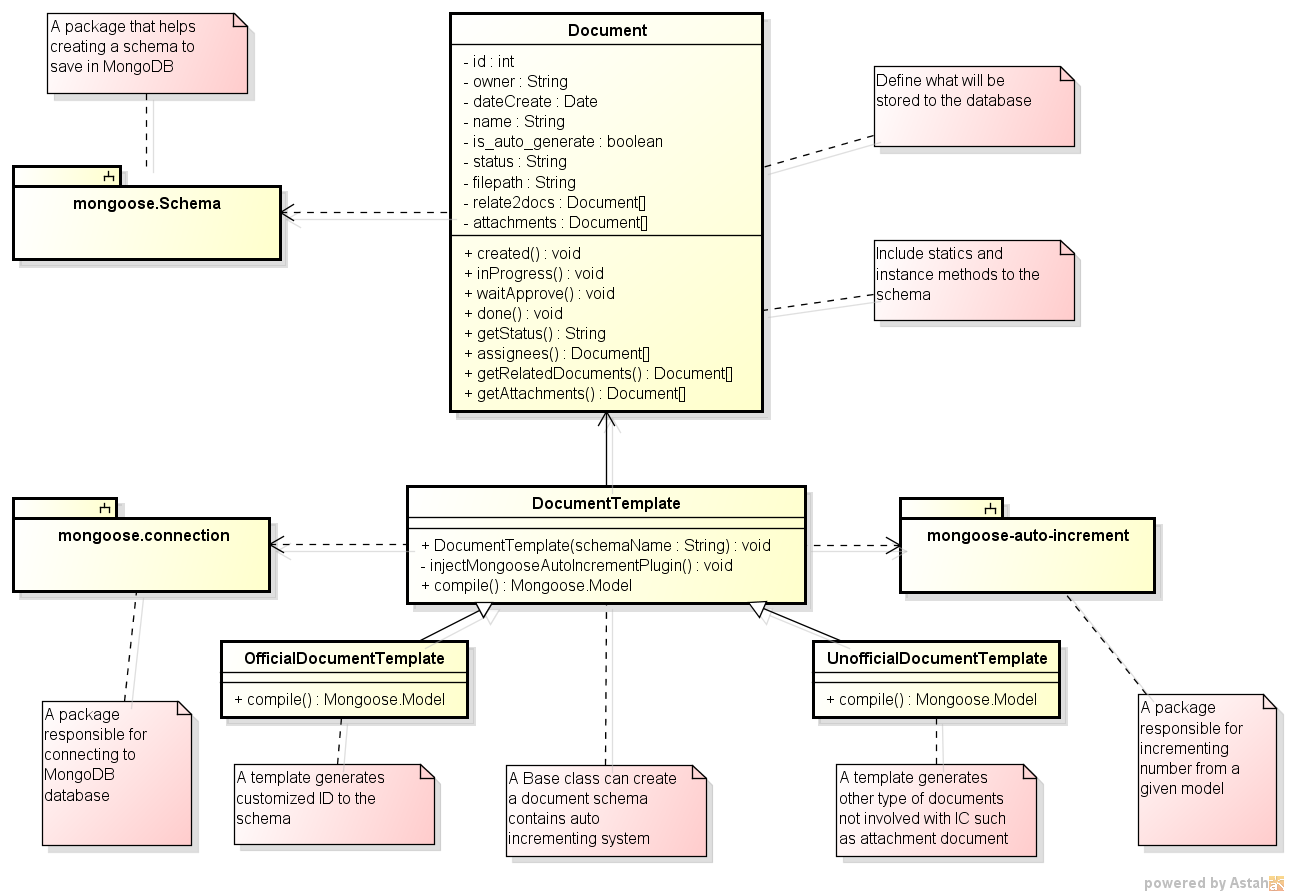
\includegraphics[scale=0.5]{res/software-design/document_templating}
\end{figure}

\textit{Document} defines attributes that represent a document.
Table \ref{uml:document-templating} describes what each attribute is, its data type, and its functionality from figure \ref{fig:doc-template}.
\begin{longtable}{lL{3cm}L{7.5cm}}
	\caption{Description of each attribute in \textit{Document} class}
	\label{uml:document-templating} \\
	\hline
	Attribute & Data type & Description \\
	\hline
	\endfirsthead
	
	\hline
	Attribute & Data type & Description \\
	\hline
	\endhead
	
	\hline \multicolumn{3}{r}{{Continued on next page}} \\ \hline
	\endfoot
	
	\hline \hline
	\endlastfoot
	
	id & String & Document identification \\
	
	owner & String & The original user who create the document. \\
	
	dateCreate & Date & A date when this record is created. \\
	
	name & String &
	The filename including extension that is going to appear on the page.
	It is the original filename that user uploaded.
	If it is a by-product from the workflow, the system automatically generates it. \\
	
	is\_auto\_generate & Boolean &
	A boolean indicates whether this document is created by the system. \\
	
	status & String & 
	Indicates the current states document going through the workflow. \\
	
	filepath & String &
	Absolute path to the file stored in a server. \\
	
	relate2Docs & array of \textit{Document} &
	Additional documents that involved with this document.
	If this document refer to other documents, they will be shown here. \\
	
	attachments & array of \textit{Document} &
	Other required documents or other dependent documents. \\
\end{longtable}

A schema has to be defined first in order to record document's metadata to the database.
The schema relies on a \textit{mongoose.Schema} package.
It provides utility for defining fields and data types suitable for saving to the database.
As the requirement states that attachments are also document.
\textit{relate2docs} and \textit{attachments} are fields that store additional documents.
They should have \textit{Document} data type.
Setting them this way provides a benefit that all metadata about attachments and related documents can be queried from the same object.

\textit{Document} class also defines methods to manipulate the schema which are its attributes.
Table \ref{uml:document-method} describes each method in detail.

\begin{longtable}{lL{2.5cm}L{7.5cm}}
	\caption{\textit{Document} methods}
	\label{uml:document-method} \\
	\hline
	Method & Return data type & Description \\
	\hline
	\endfirsthead
	
	\hline
	Method & Return data type & Description \\
	\hline
	\endhead		
	
	\hline \multicolumn{3}{r}{{Continued on next page}} \\ \hline
	\endfoot
	
	\hline \hline
	\endlastfoot
	
	created & &  Set document's status for newly created document. \\
	inProgress & & Set document's status as processing. \\
	done & & Set document's status as done. \\
	waitApprove & & Set document's status as waiting approval \\
	getStatus & String & Get the current status on this document. \\
	getRelatedDocuments & array of \textit{Document} & Get all related documents. \\
	getAttachments & array of \textit{Document} & Get all attachments. \\
\end{longtable}

\textit{DocumentTemplate} applies auto increment functionality to the schema.
Every time the schema is saved, it invokes the auto increment functionality automatically.
In design pattern, \textit{DocumentTemplate} is a factory that creates instance object according to given parameters.
There are two subclasses inherits \textit{DocumentTemplate}, \textit{OfficialDocumentTemplate} and \textit{UnOfficialDocumentTemplate}.
\textit{OfficialDocumentTemplate} creates a document template based on a given type name and year.
They are used to create a document with custom identification code as stated in table \ref{tbl-doc-subtype}.
The purpose of \textit{UnOfficialDocumentTemplate} is to create external documents and attachments.
It has the same functionality as \textit{DocumentTemplate}.
Table \ref{uml:document-template} explains what each method does.

\begin{longtable}{L{4cm}L{2.5cm}L{7.5cm}}
	\caption{\textit{DocumentTemplate} description}
	\label{uml:document-template} \\
	\hline
	Method & Return data type & Description \\
	\hline
	\endfirsthead
	
	\hline
	Method & Return data type & Description \\
	\hline
	\endhead		
	
	\hline \multicolumn{3}{r}{{Continued on next page}} \\ \hline
	\endfoot
	
	\hline \hline
	\endlastfoot
	
	OfficialDocumentTemplate & & A class constructor that receives document type and year to generate an identification code. \\
	
	injectMongooseAutoIncrementPlugin & &  Inject \textit{mongoose-auto-increment} package to the schema as a plugin so that the schema can increment the number every time before saving the database. \\
	
	compile & \textit{mongoose.model} & Create a model from a schema because the \textit{mongoose.Schema} package requires \textit{mongoose.connection} in order to prepare the schema suitable for saving to the database.
\end{longtable}

\section{Retrieving Digital Documents}
Retrieving digital documents means querying recorded metadata from the database.
Referring to figure \ref{fig:doc-template}, the \textit{id} field in \textit{Document} class is a field with unique value.
The system can query a specific document using the \textit{id} field.
The system can also use \textit{owner} field to search documents owned by a specific user.
Fortunately, \textit{mongoose.Model} package encapsulates database layer.
Each record in the database is treated as an object.
After querying from the database, it assigns results to each field and instantiate an object from the \textit{Document} class automatically.

\section{Rejecting and Approving Digital Documents}

\section{Mock-up}

\section{Development Tools}
